\begin{figure}[th]
\centering
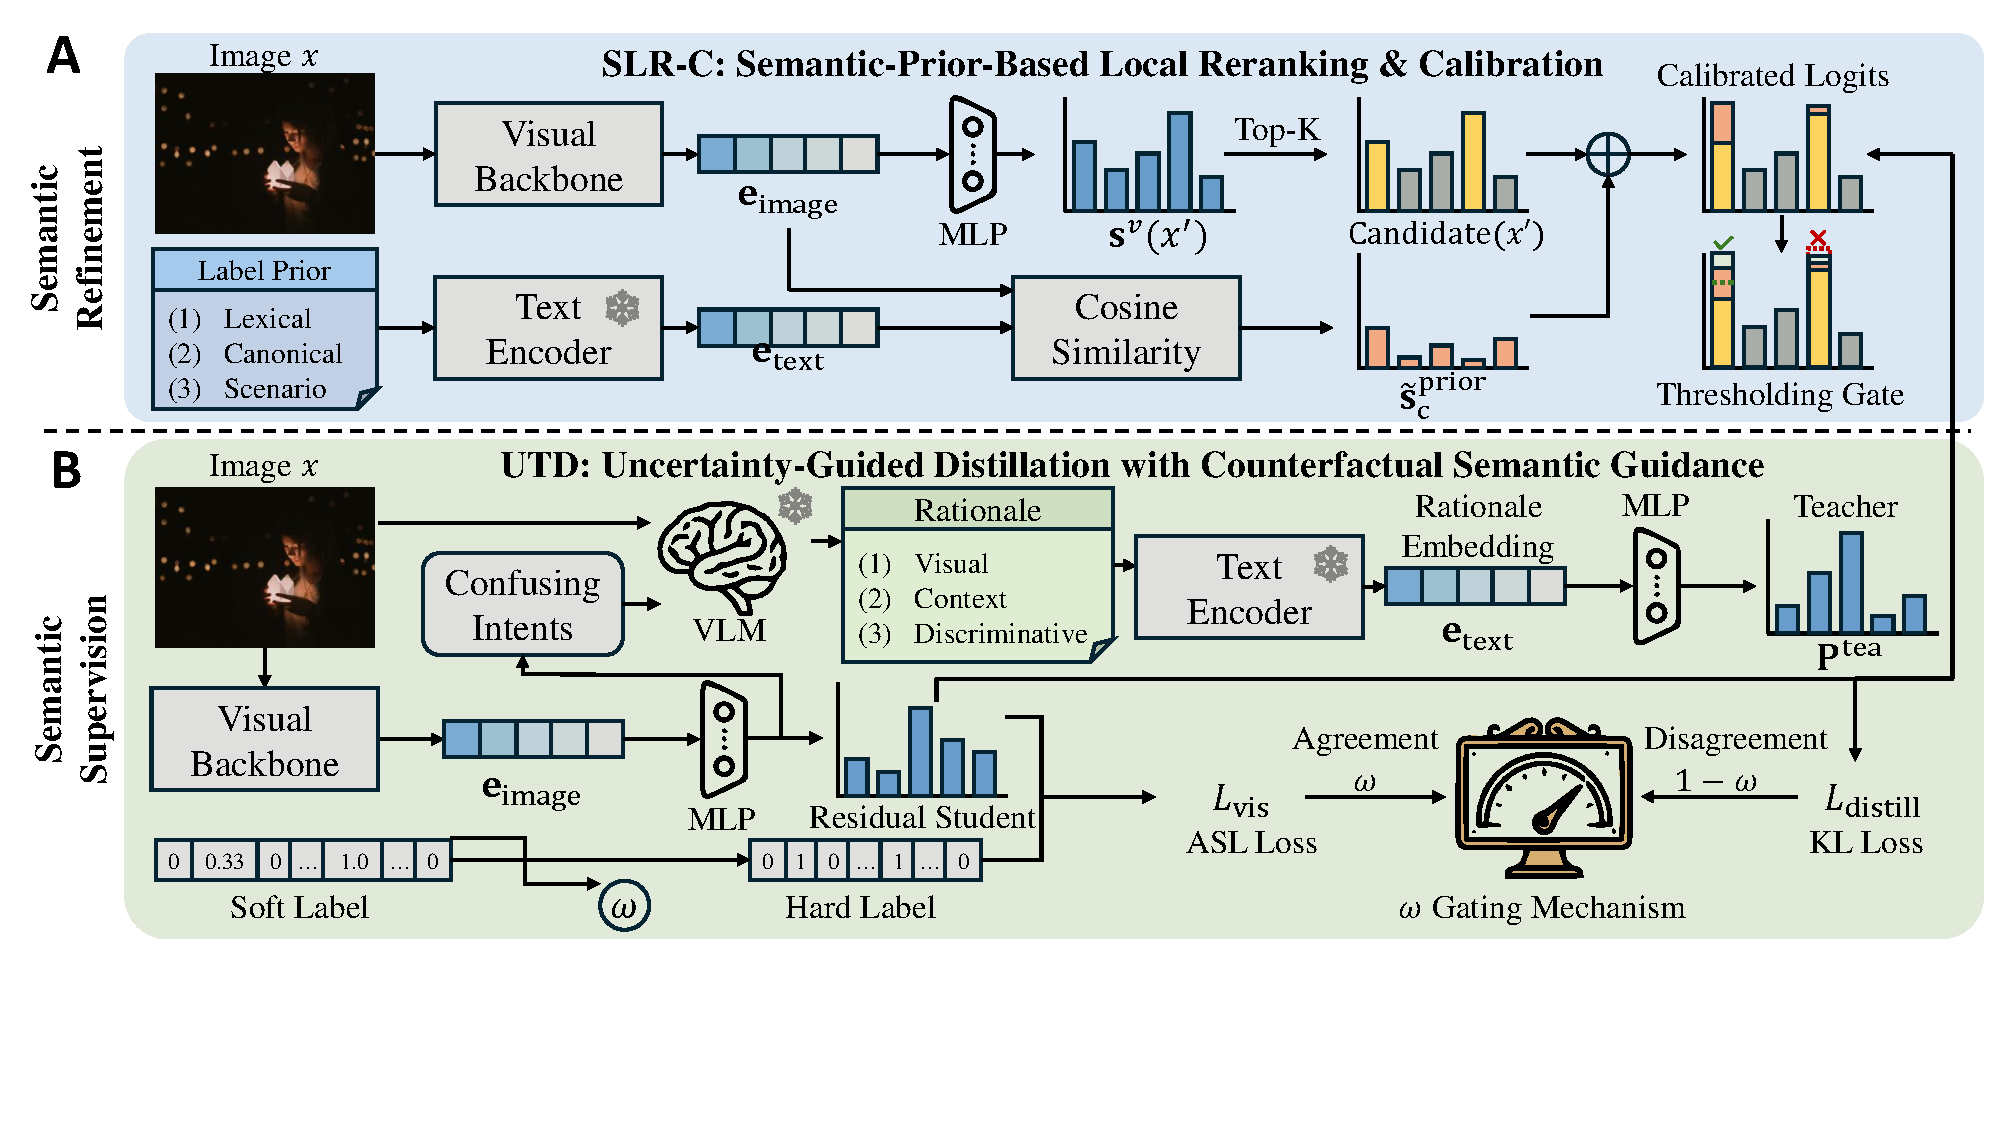
\includegraphics[width=\linewidth]{srcs/framework.pdf}
\caption{Overview of the FDIL framework. The framework functionally decouples ambiguity handling into \textbf{semantic refinement} and \textbf{semantic supervision}. \textbf{(Bottom) SLR-C module:} heterogeneous lexical, canonical, and scenario priors define a semantic prior through Top-$K$ reranking, after which a lightweight residual student adapts the final prediction to image evidence before class-wise calibration. \textbf{(Top) UTD module:} a VLM-derived text teacher provides rationale-based semantic supervision, and its contribution is adaptively gated by the annotator agreement score $\omega$ to stabilize learning under supervisory ambiguity.}
\label{fig:fdil_framework}
\end{figure}

\section{Method}
\label{sec:method}

\subsection{Overview}

To address the dual challenges of supervisory ambiguity and semantic ambiguity in visual intention recognition, we propose \textbf{FDIL}, a functionally decoupled framework where fixed semantic priors provide structured candidate semantics, uncertainty-aware text teachers stabilize ambiguous supervision, and a residual student learns image-aware intent prediction on top of the semantic prior. Instead of forcing one unified mechanism to handle both supervisory ambiguity and semantic ambiguity, we assign them to two complementary functions.

FDIL consists of two key components, as shown in Figure~\ref{fig:fdil_framework}:
\begin{itemize}
    \item \textbf{Semantic Local Reranking and Calibration (SLR-C)}, which constructs a semantic prior from heterogeneous textual cues and supports image-aware refinement through a residual student;
    \item \textbf{Uncertainty-guided Text Distillation (UTD)}, which introduces adaptive semantic guidance to improve robustness under ambiguous supervision;
\end{itemize}

Given an input image, the model first produces visual intent scores using a strong visual backbone. SLR-C then provides structured candidate semantics by locally reranking intent candidates and forming a semantic prior. UTD supplies uncertainty-aware semantic supervision through a rationale-based text teacher and can be reused to regularize both the visual student and the residual refinement module built on top of the semantic prior.

\subsection{Problem Formulation}

Given an input image $x$, the goal is to predict a set of intent labels from a predefined label space $\mathcal{Y}=\{1,\dots,C\}$. Due to the subjective nature of visual intention recognition, annotations are provided as soft label vectors $\mathbf{y}^{\text{soft}} \in \{0, 0.33, 0.66, 1\}^C$, reflecting annotator agreement.

Existing approaches typically follow either hard binarization or soft regression paradigms, both of which have limitations under ambiguous supervision. To address this, we adopt a \textbf{decoupled utilization} of annotation signals.

Specifically, we derive binarized labels $\mathbf{y}^{\text{hard}}$ for classification supervision, while extracting an image-level agreement score $\omega \in (0,1]$ from $\mathbf{y}^{\text{soft}}$. Here, $\omega$ reflects annotator consensus, where higher values indicate more reliable supervision. The binarized labels are computed as:
\begin{equation}
y^{\text{hard}}_{c} =
\begin{cases}
1, & \text{if } y^{\text{soft}}_{c} > 0 \\
0, & \text{otherwise}
\end{cases}
\end{equation}

In practice, an image may contain multiple positive intents with different agreement levels. We therefore adopt a conservative pooling rule and define the sample-level agreement as the minimum soft agreement among all positive labels:
\begin{equation}
\omega = \min_{c:\, y^{\text{hard}}_{c}=1} y^{\text{soft}}_{c}.
\end{equation}
This choice lets the hardest positive label determine how much the sample should trust direct supervision.

\subsection{Semantic Local Reranking and Calibration (SLR-C)}

Semantic ambiguity mainly manifests as local confusion among visually plausible but semantically adjacent intents. To address this, we first build a semantic refinement module that provides structured candidate semantics before turning to ambiguity-aware supervision.

\subsubsection{Semantic Prior Construction}

Intent semantics are inherently multi-granular and abstract, making a single textual representation insufficient. We therefore construct a heterogeneous semantic prior for each intent by combining three complementary textual sources: lexical intent phrases, canonical intent descriptions, and descriptive visual scenarios. The lexical source provides concise intent name cues, the canonical source provides semantic definitions, and the scenario source grounds abstract intents into plausible visual situations.

Given an image $x$, we compute image-text similarities:
\begin{equation}
s^{\text{prior}}_c = \text{sim}(f_{\text{img}}(x), \mathbf{e}_c).
\end{equation}
In practice, $\text{sim}(\cdot,\cdot)$ is cosine similarity between L2-normalized image and text embeddings, scaled by the CLIP logit scale $\gamma$, i.e.
\begin{equation}
\text{sim}(f_{\text{img}}(x), \mathbf{e}_c) = \gamma \cdot \frac{f_{\text{img}}(x)^\top \mathbf{e}_c}{\|f_{\text{img}}(x)\|_2 \|\mathbf{e}_c\|_2}.
\end{equation}

For each source, we obtain a class-wise similarity score and normalize it independently. Specifically, for source $r \in \{\text{lex}, \text{can}, \text{scen}\}$, we perform per-sample normalization across all classes:
\begin{equation}
\tilde{s}^{r}_c = \frac{s^{r}_c - \mu^{r}(x)}{\sigma^{r}(x) + \epsilon},
\end{equation}
where $\mu^{r}(x)=\frac{1}{C}\sum_{c=1}^{C}s^{r}_c$ and $\sigma^{r}(x)$ is the corresponding standard deviation over the $C$ intent classes, with $\epsilon$ a small constant for numerical stability. The final prior is then constructed by averaging the normalized scores from the three sources:
\begin{equation}
\tilde{s}^{\text{prior}}_c = \frac{1}{3}\left(\tilde{s}^{\text{lex}}_c + \tilde{s}^{\text{can}}_c + \tilde{s}^{\text{scen}}_c\right).
\end{equation}

\subsubsection{Semantic Local Reranking}

In the refinement module, we start from base visual logits $\mathbf{s}^{b}$ produced by a frozen visual student. We first select a compact candidate set:
\begin{equation}
\mathcal{C}_K(x) = \text{TopK}(\mathbf{s}^{b}, K).
\end{equation}

The base logits are then locally adjusted with the normalized prior:
\begin{equation}
\tilde{s}_c =
\begin{cases}
s^{b}_c + \alpha \cdot \tilde{s}^{\text{prior}}_c, & c \in \mathcal{C}_K(x), \\
s^{b}_c, & \text{otherwise}.
\end{cases}
\end{equation}
Here $\alpha$ controls the strength of semantic reranking. In our implementation, $\alpha$ is fixed to 0.3.

This localized reranking produces a semantic prior that narrows the candidate set and sharpens the local score geometry without introducing an additional trainable prior module.

\subsubsection{Residual Refinement on the Semantic Prior}

Fixed reranking alone is not sufficient, because the heterogeneous prior may still fall short of the image-specific evidence. We therefore train a lightweight residual student on top of the semantic prior:
\begin{equation}
s^{\text{full}}_c = \tilde{s}_c + h_{\text{res}}(f_{\text{img}}(x))_c,
\end{equation}
where $h_{\text{res}}(\cdot)$ is a residual MLP that predicts class-wise residual intent scores from the image feature. In practice, the SLR-C logits $\tilde{\mathbf{s}}$ are first computed and frozen, and the residual module is then optimized separately.

In the final full model, this residual module is not trained in isolation: it can also be regularized by the uncertainty-aware text teacher introduced next. Thus, SLR-C provides the structured candidate semantics first, and UTD later supplies the ambiguity-aware supervision used to stabilize image-aware prediction on top of the semantic prior.

\subsubsection{Class-wise Calibration}

To account for class imbalance and varying score distributions, we adopt class-wise thresholds:
\begin{equation}
\hat{y}_c = \mathbb{I}[\sigma(s^{\text{full}}_c) > t_c],
\end{equation}
where $t_c$ is determined on the validation set. Concretely, each threshold is selected independently by maximizing the class-wise validation F1:
\begin{equation}
t_c^\ast = \arg\max_{t \in \mathcal{T}} \text{F1}_c^{\text{val}}(t),
\end{equation}
where $\mathcal{T}$ is a fixed threshold grid. This design lets each class adapt its decision boundary to its own score distribution and frequency level, instead of sharing a single global threshold.

\subsection{Uncertainty-guided Text Distillation (UTD)}

\subsubsection{Motivation}

Supervisory ambiguity arises when multiple plausible intents coexist for a given image. Direct optimization against hard labels may lead to overconfident predictions and unstable decision boundaries. To alleviate this issue, we introduce semantic guidance from text space and adapt its influence based on the uncertainty of supervision.

\subsubsection{Text-derived Teacher}

For each training image, we construct structured textual descriptions that capture semantic cues relevant to intention understanding. These descriptions are generated offline by a vision-language model, guided by both the image content and intent semantics.

To enhance discriminative capability under semantic ambiguity, we further incorporate contrastive cues by identifying visually plausible but incorrect intents predicted by the current model. Specifically, we select high-confidence negative intents as confusion candidates and use them to guide the generation of discriminative textual descriptions. This encourages the resulting text to emphasize subtle distinctions among semantically adjacent intents.

The generated text aims to summarize three aspects:
(1) observable visual elements,
(2) contextual interpretation beyond direct perception, and
(3) discriminative cues for distinguishing confusing intents.

The resulting text $T(x)$ is encoded into a dense embedding space using a frozen text encoder:
\begin{equation}
\mathbf{e}_{\text{text}} = f_{\text{text}}(T(x)).
\end{equation}

A lightweight classifier then maps the embedding into a multi-label teacher distribution:
\begin{equation}
\mathbf{p}^{\text{tea}} = \sigma(g_{\text{tea}}(\mathbf{e}_{\text{text}}) / \tau),
\end{equation}
where $\sigma(\cdot)$ is the sigmoid function and $\tau$ is the temperature parameter.

This design introduces contrastive semantic signals that improve the teacher's ability to distinguish semantically similar intents, while remaining separate from the semantic prior itself. In the full FDIL pipeline, the same teacher can further regularize the residual refinement module built on top of SLR-C.

\subsubsection{Uncertainty-guided Distillation}

The visual backbone produces logits $\mathbf{s}^{v}$ for image $x$. We adopt Asymmetric Loss \cite{ridnik_asymmetric_2021} for classification:
\begin{equation}
\mathcal{L}_{\text{vis}} = \frac{1}{C} \sum_{c=1}^{C} \ell_{\text{ASL}}(s^{v}_{c}, y^{\text{hard}}_{c}).
\end{equation}

To incorporate semantic guidance, we introduce an uncertainty-guided Bernoulli distillation loss:
\begin{equation}
\mathcal{L}_{\text{distill}} = \sum_{c=1}^{C}\text{KL}\big(\sigma(s_c^{v}/\tau)\,\|\, p_c^{\text{tea}}\big),
\end{equation}
which is applied independently to each label. We use Bernoulli-style distillation rather than softmax distillation because intent recognition is a multi-label problem and class probabilities are not mutually exclusive. Here, $\lambda$ denotes the distillation weight that controls the overall contribution of the teacher signal relative to the visual supervision term. In our experiments, $\lambda$ is fixed to 1.0.

Rather than mixing the two objectives with a fixed global coefficient, we use a gate derived from the agreement score. For the current sample, the teacher branch weight is defined as $g = 1 - \omega$ so low-agreement samples receive stronger semantic guidance, while high-agreement samples remain dominated by direct visual supervision.

Using $g$, the final loss is
\begin{equation}
\mathcal{L}_{\text{total}} = (1-g)\mathcal{L}_{\text{vis}} + \lambda g \mathcal{L}_{\text{distill}}
= \omega \mathcal{L}_{\text{vis}} + \lambda (1-\omega)\mathcal{L}_{\text{distill}}.
\end{equation}

This gated formulation allows the model to rely more on visual supervision when annotations are reliable, and to leverage semantic guidance when supervision is uncertain. In other words, UTD stabilizes ambiguous supervision through an uncertainty-aware text teacher rather than by modifying the semantic prior itself.

\subsection{Functionally Decoupled Ambiguity Modeling}

We interpret visual intention recognition as a functionally decoupled ambiguity problem. Semantic ambiguity primarily distorts local candidate semantics, while supervisory ambiguity primarily destabilizes semantic supervision.

FDIL addresses these two aspects through two different but compatible functions: SLR-C first provides structured candidate semantics through a semantic prior and residual refinement, while UTD supplies agreement-guided semantic supervision that stabilizes both the visual student and, in the full model, the residual refinement module built on top of the prior. This formulation is faithful to the current implementation, where the refinement module is optimized separately rather than jointly end-to-end with the teacher module.

This functionally decoupled design enables effective handling of ambiguity without introducing heavy architectural complexity.
